\section{Remise en contexte}
\subsection{Pr�sentation de l'entreprise}
\begin{frame}
  \frametitle{Pr�sentation de l'entreprise}
  \textbf{SEW Usocome}

  \begin{minipage}{.5\textwidth}
  \begin{itemize}
  \item filiale fran�aise du groupe allemand \textbf{SEW-EURODRIVE}
  \item usines � Haguenau, Brumath et Forbach
  \item propose des solutions d'automatisme pour des applications de
    mouvement (moteur �lectrique, servomoteur..)
  \end{itemize}
\end{minipage}%
\begin{minipage}{.5\textwidth}
  \begin{figure}
    \centering
    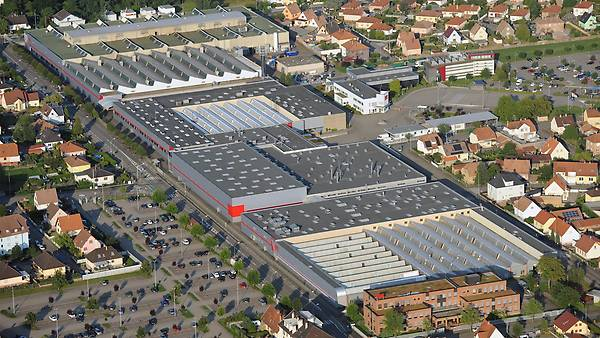
\includegraphics[scale=1,width=0.9\textwidth]{sew_haguenau.jpg}
    \caption{Vue de l'usine de Haguenau}
    \label{fig:sew_haguenau}
  \end{figure}
\end{minipage}
\end{frame}
%
% %%%% --4--%%%%
\subsection{Etat actuel}
\begin{frame}
  \frametitle{Etat actuel}

  Gestion des stocks inexistantes entre les zones de production et de
  stockage et les autres usines.

  \textbf{Probl�matique~:} Avoir constamment des contenants vides sur
  les zones de production et suffisamment de contenants utiles � la
  production sur chaque site

  \begin{minipage}{.5\textwidth}
    \begin{figure}
      \centering
      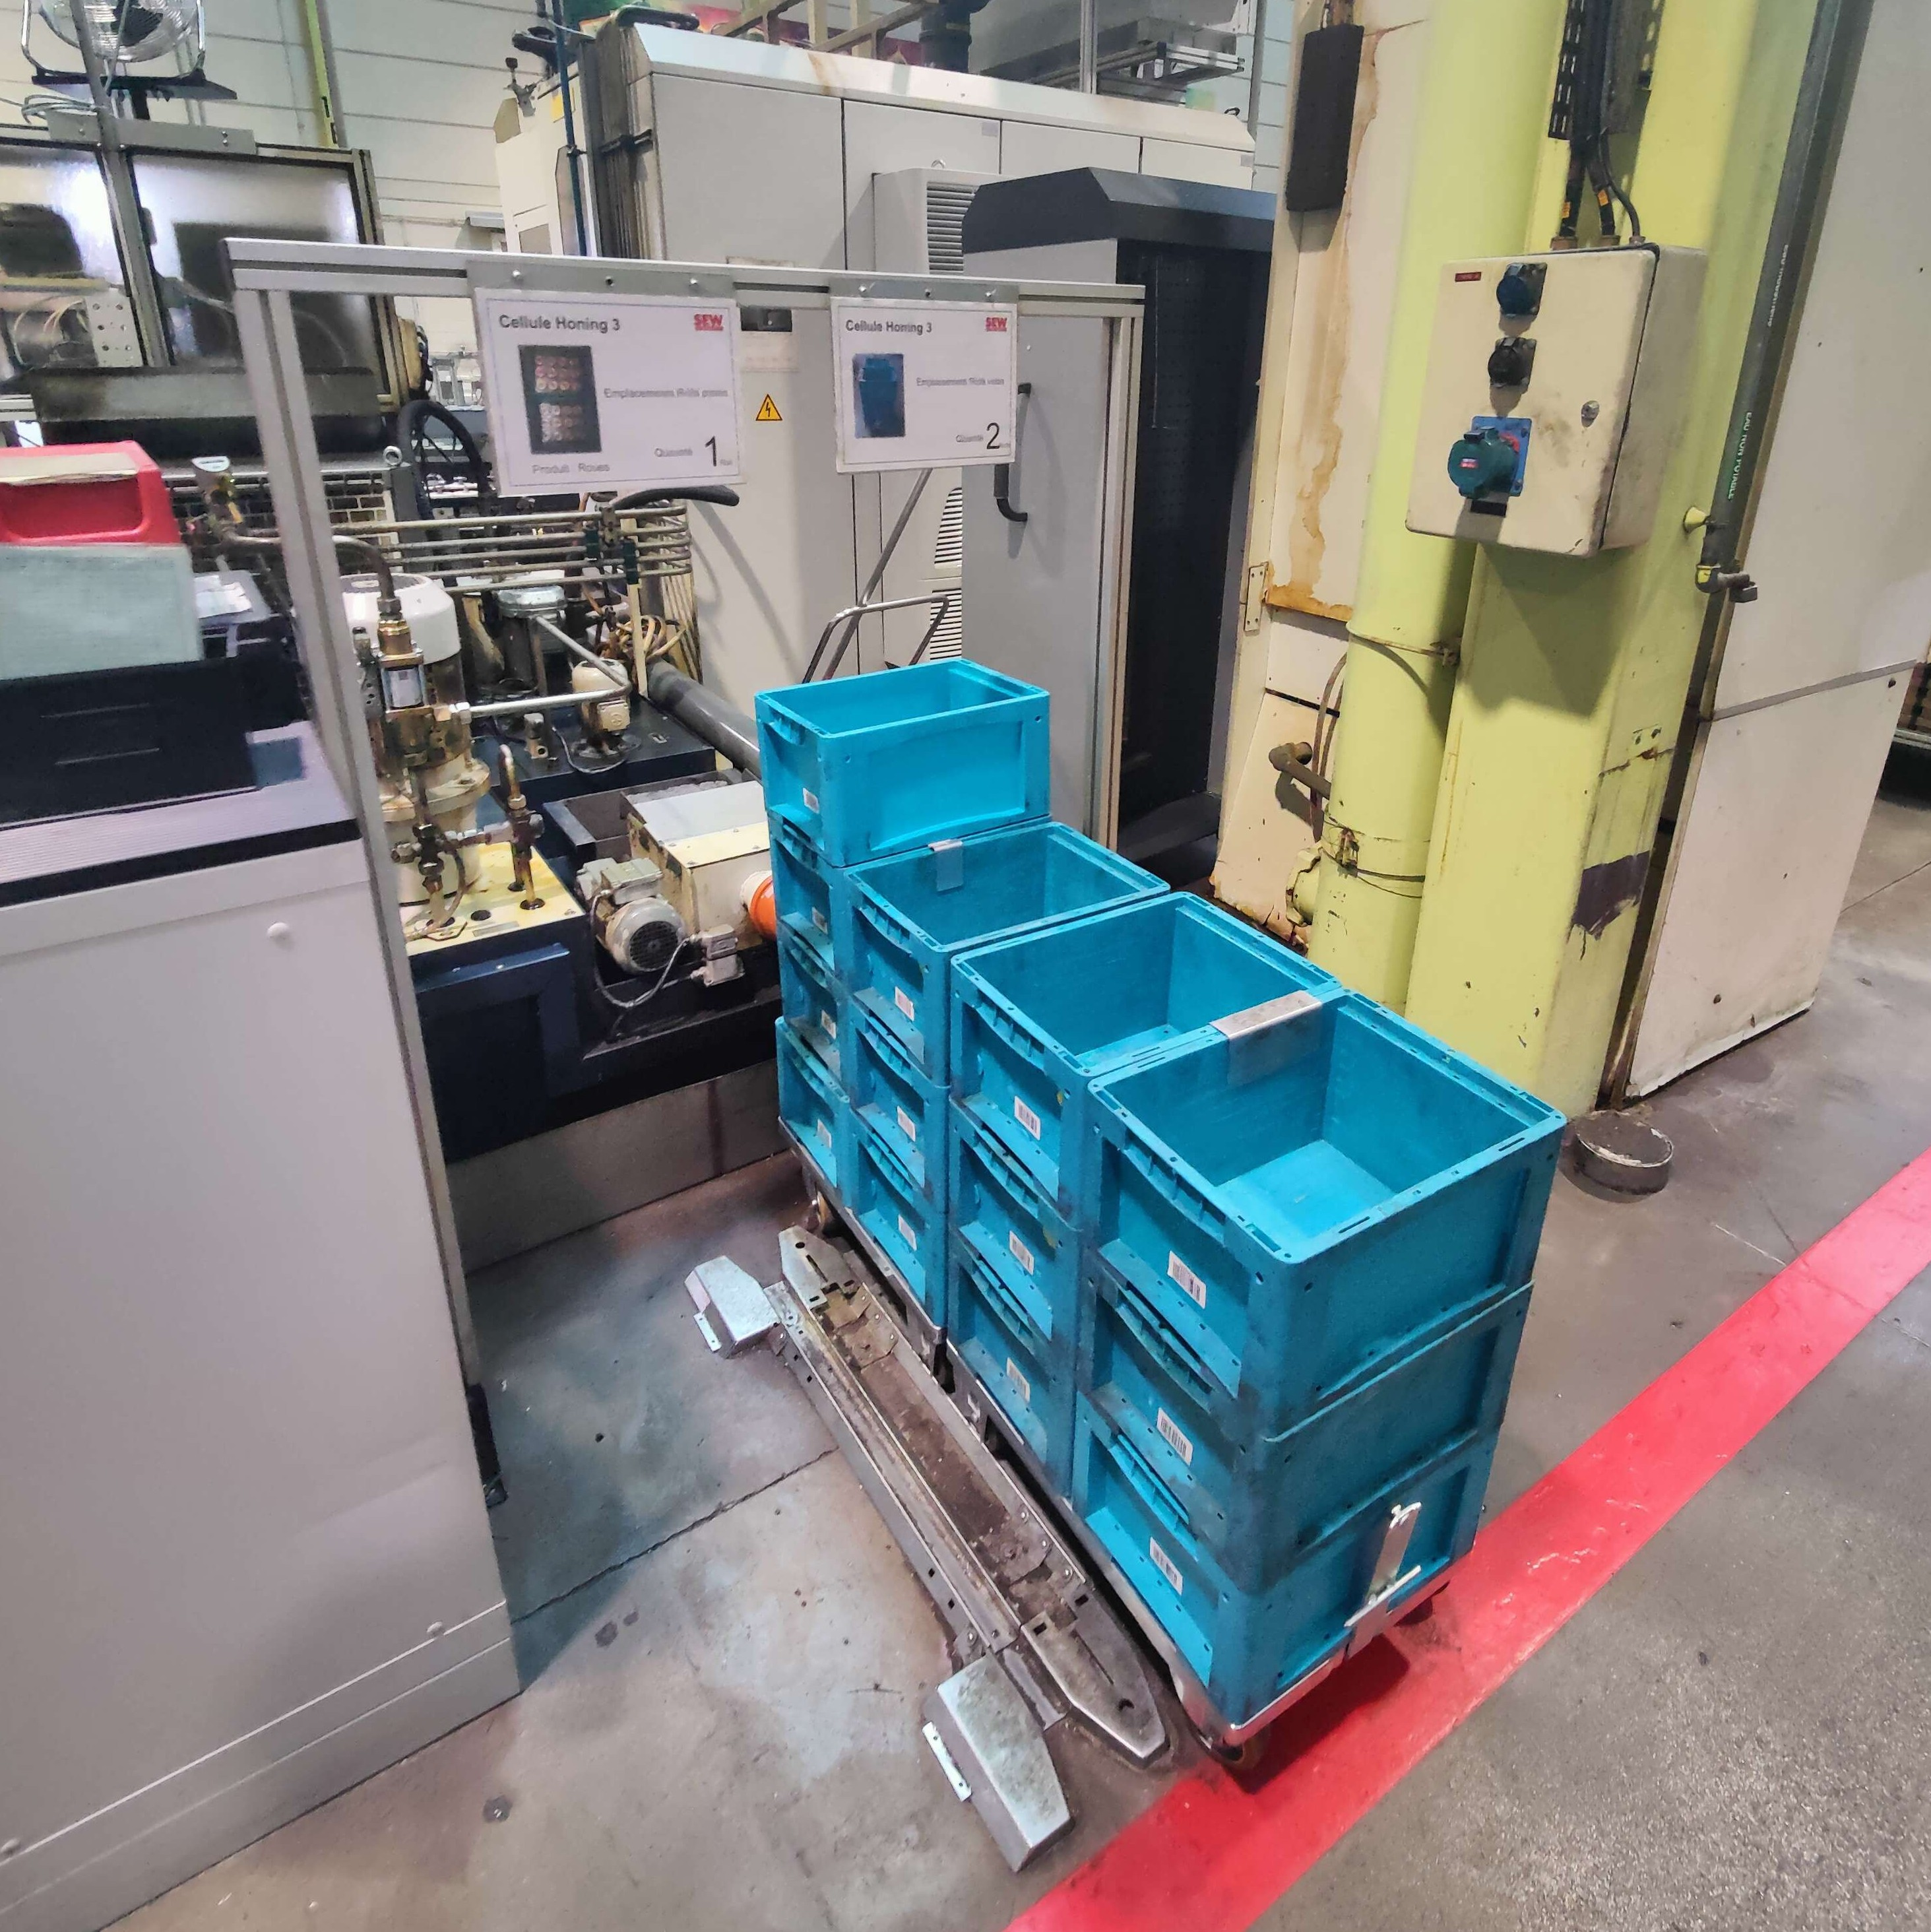
\includegraphics[width=0.7\textwidth, height=0.47\textheight]{sew_production.jpg}
      \caption{Image d'une zone de production d'Haguenau}
      \label{fig:sew_production}
    \end{figure}
  \end{minipage}%
  \begin{minipage}{.5\textwidth}
    \begin{figure}
      \centering
      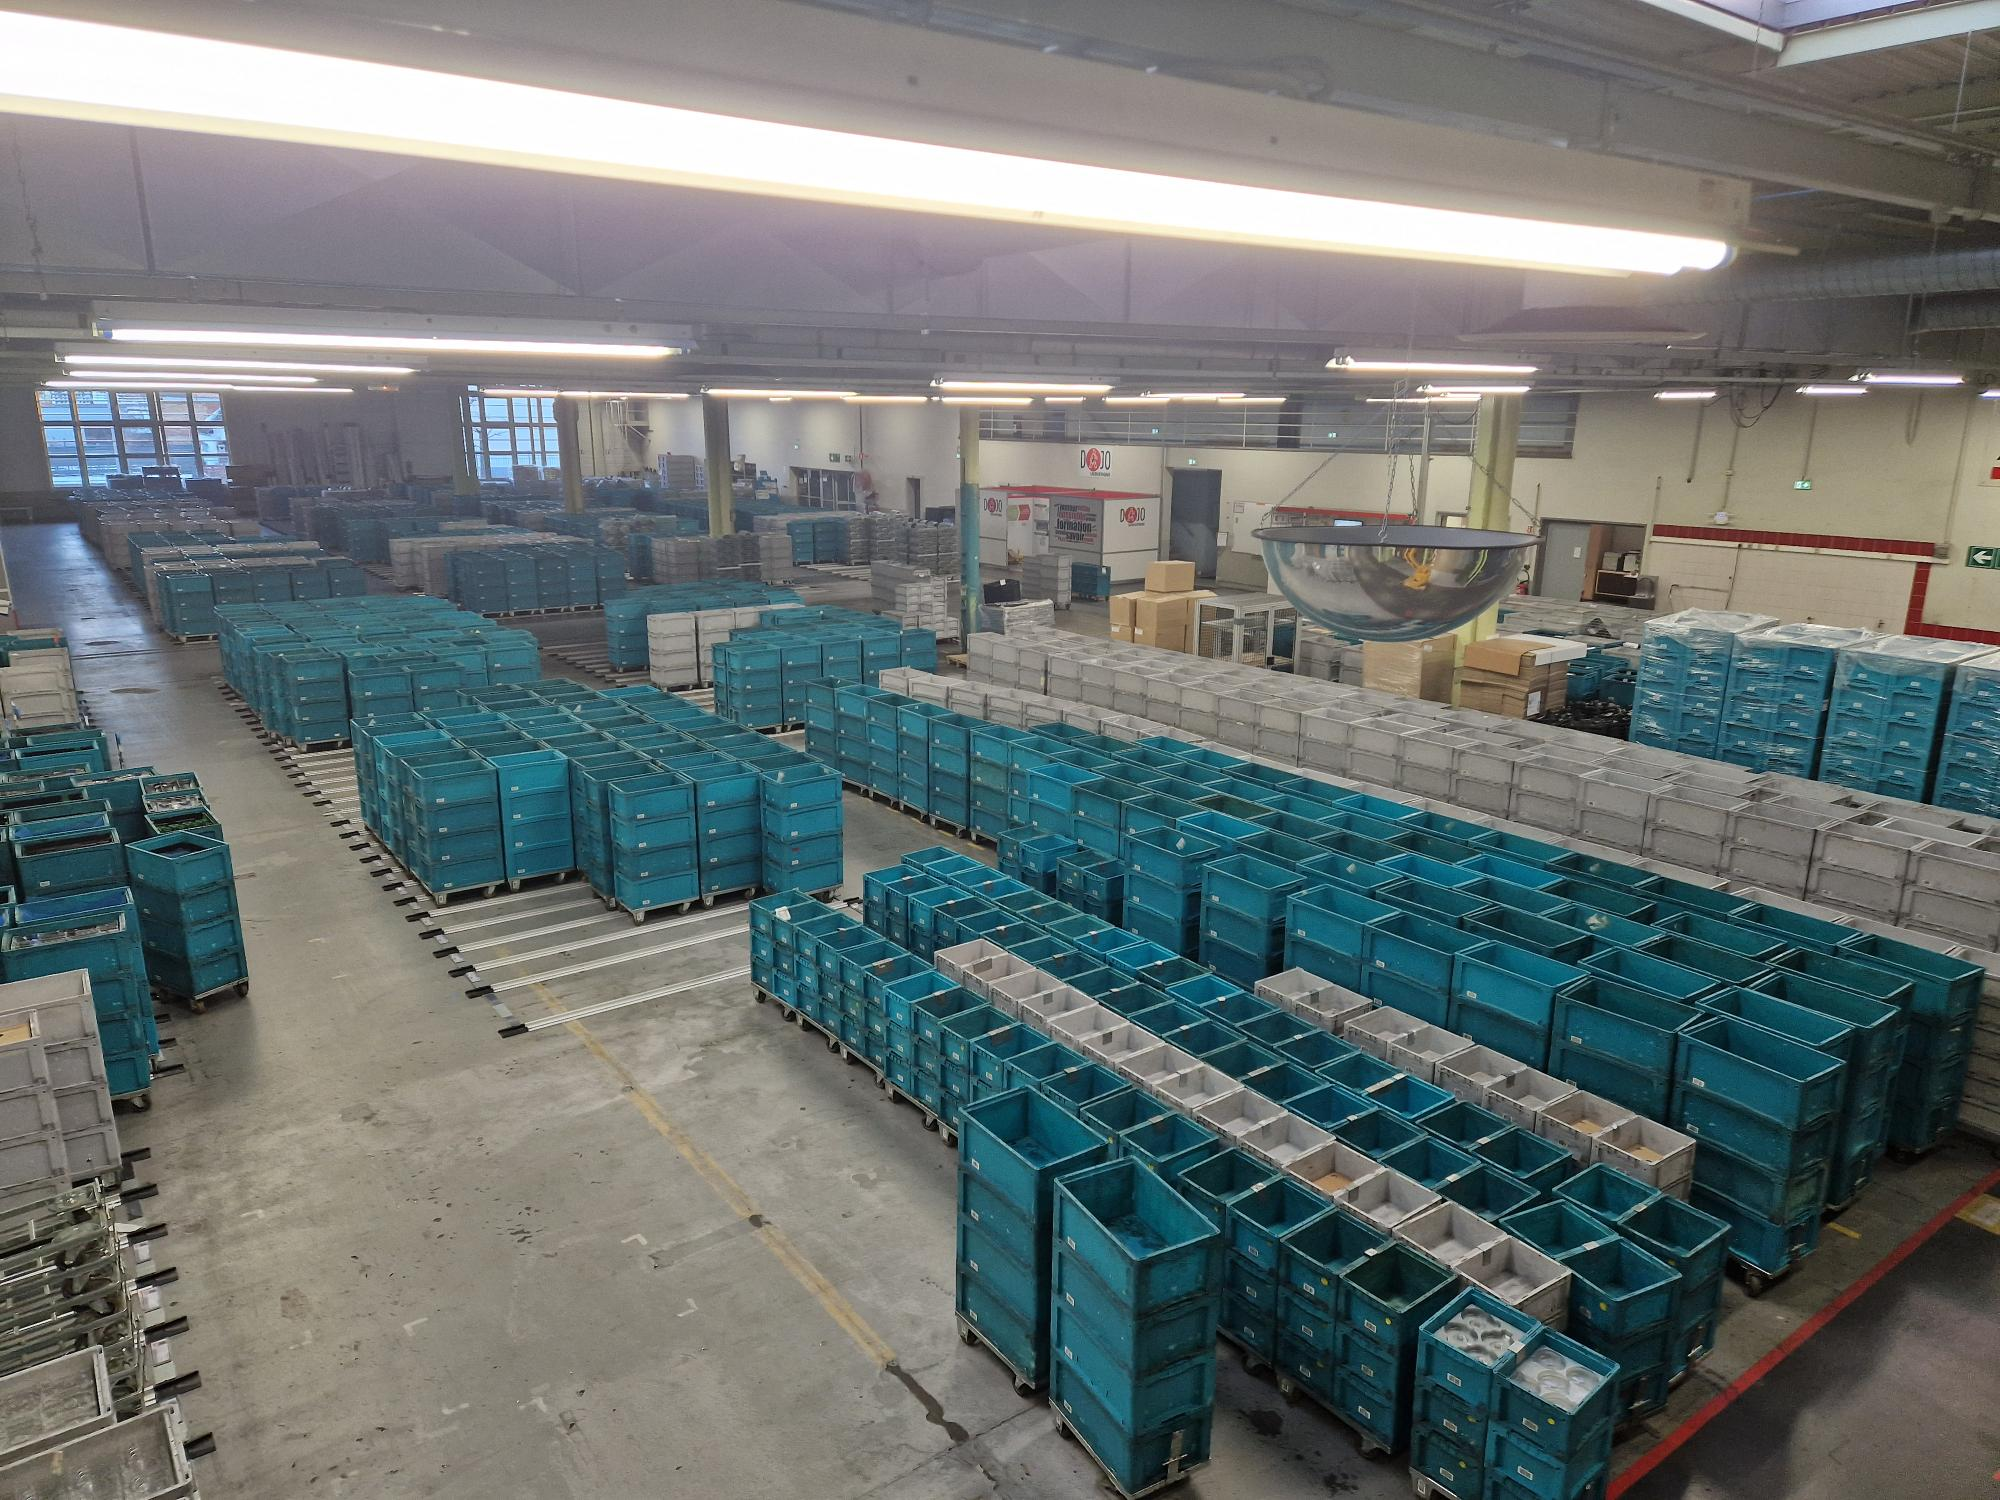
\includegraphics[scale=1,width=0.9\textwidth]{sew_entrepot.jpg}
      \caption{Image de la zone de stockage de Haguenau}
      \label{fig:sew_entrepot}
    \end{figure}
  \end{minipage}
\end{frame}%
%
% %%% --5--%%%
\subsection{Objectifs du projet}
\begin{frame}
  \frametitle{Objectifs du projet}
  \textbf{Objectif principal~:} Classification et comptage des
  contenants vides

  % \begin{tabular}{|p{1ex}|p{1ex}|p{1ex}|}
  %   \hline
  %   Objectifs & Crit�res & Moyens\\
  %   \hline
  %   Classification des bo�tes par apprentissage automatique & Avoir
  %                                                             environ
  %                                                             90  de
  %                                                             pr�cision
  %                        & Utiliser Python et YOLO\\
  %   \hline
  % \end{tabular}
\end{frame}
%